% Preambulo compartido para clases en formato beamer
\documentclass[9pt, xcolor=svgnames]{beamer}
\usepackage[utf8]{inputenc}
\usepackage[T1]{fontenc}
\usepackage[spanish,es-nodecimaldot]{babel}

\usetheme[progressbar=frametitle]{metropolis}
\metroset{sectionpage=none, subsectionpage=none}
\usepackage{appendixnumberbeamer}
\usepackage{booktabs}
\usepackage{amsmath,amssymb,bm,mathtools}
\usepackage{physics}
\usepackage{graphicx}
\usepackage{multicol}
\usepackage{tikz}
\usepackage{minted}
\usemintedstyle{tango}
\setminted{fontsize=\scriptsize, breaklines=true, linenos=true, bgcolor=LightGray!20, frame=lines}
\newminted{python}{fontsize=\scriptsize, breaklines=true, linenos=true, bgcolor=LightGray!20, frame=lines}
\usepackage{pgfplots}
\pgfplotsset{compat=1.18}
\usepackage{ragged2e}
\usepackage{xspace}
\newcommand{\themename}{\textbf{\textsc{metropolis}}\xspace}

\setbeamercolor{block title}{bg=MidnightBlue!85, fg=white}
\setbeamercolor{block body}{bg=MidnightBlue!5, fg=black}
\setbeamercolor{alerted text}{fg=Crimson}
\setbeamercolor{frametitle}{bg=MidnightBlue!10, fg=black}
\setbeamertemplate{blocks}[rounded][shadow=true]


\weektitle{11}{redes convolucionales con keras}
\titlegraphic{}
\title[PCFI261 -- Semana 11]{\Large Modelos Computacionales PCFI261\\Semana 11: redes convolucionales\\con Keras}
\newcommand{\compactcode}{\fontsize{5.35}{5.1}\selectfont}
\setminted[python]{
    fontsize=\compactcode,
    breaklines=true,
    breakanywhere=true,
    linenos=true,
    numbersep=3pt,
    bgcolor=LightGray!12,
    frame=single,
    framesep=1.1mm,
    rulecolor=MidnightBlue!55,
    baselinestretch=0.78,
    tabsize=2
}

\begin{document}

\begin{frame}[plain]
\centering
\vfill
{\Large\bfseries Modelos Computacionales PCFI261}\\[0.25cm]
{\large Semana 11: redes convolucionales\\con Keras}\\[0.7cm]
{\large Joaquin Peralta}\\[0.15cm]
{\small \texttt{joaquin.peralta@unab.cl}}\\[0.35cm]
{\small Universidad Andres Bello}
\vfill
\end{frame}

\begin{frame}{Organizacion de la semana}
\begin{block}{Continuidad desde semanas 09 y 10}
Venimos de redes densas para datos tabulados, emuladores fisicos y senales astronomicas. Esta semana cambiamos el tipo de dato: imagenes. La pregunta central es por que una red densa funciona razonablemente, pero una CNN aprovecha mejor la estructura espacial.
\end{block}

\begin{columns}[T,onlytextwidth]
\column{0.48\textwidth}
\textbf{Clase 1}
\begin{itemize}
    \item MNIST como laboratorio controlado;
    \item red densa simple como linea base;
    \item evaluacion de errores y confianza;
    \item limites de aplanar una imagen.
\end{itemize}

\column{0.48\textwidth}
\textbf{Clase 2}
\begin{itemize}
    \item convoluciones, filtros y pooling;
    \item CNN pequena con \texttt{tensorflow.keras};
    \item comparacion contra la red densa;
    \item foto propia de un numero y prediccion.
\end{itemize}
\end{columns}
\end{frame}

\begin{frame}{Idea de la semana}
\begin{columns}[T,onlytextwidth]
\column{0.52\textwidth}
\begin{block}{Misma tarea, dos modelos}
Clasificaremos digitos escritos a mano. Primero usamos una red densa que mira la imagen como una lista de 784 numeros. Luego usamos una CNN que conserva la vecindad entre pixeles.
\end{block}
\begin{itemize}
    \item El dataset MNIST permite iterar rapido.
    \item La red densa sirve como benchmark docente.
    \item La CNN introduce una idea fisica: patrones locales repetidos.
    \item La foto propia muestra el salto entre dataset limpio y dato real.
\end{itemize}
\column{0.44\textwidth}
\centering
\resizebox{0.96\linewidth}{!}{\begin{tikzpicture}[scale=0.72,transform shape]
\tikzstyle{box}=[draw,rounded corners=3pt,very thick,minimum width=2.8cm,minimum height=1.05cm,align=center,font=\small\bfseries]
\node[box,fill=MidnightBlue!12,draw=MidnightBlue!70] (mnist) at (0,0) {MNIST\\$28\times28$};
\node[box,fill=ForestGreen!12,draw=ForestGreen!70] (dense) at (3.5,1.05) {red densa\\linea base};
\node[box,fill=Purple!12,draw=Purple!70] (cnn) at (3.5,-1.05) {CNN\\estructura local};
\node[box,fill=orange!15,draw=orange!85] (photo) at (7.2,0) {foto propia\\prediccion};
\draw[->,very thick,gray!75] (mnist) -- (dense);
\draw[->,very thick,gray!75] (mnist) -- (cnn);
\draw[->,very thick,gray!75] (dense) -- (photo);
\draw[->,very thick,gray!75] (cnn) -- (photo);
\node[font=\scriptsize,align=center,text width=8.2cm] at (3.6,-2.35) {Primero probamos una red simple que aplana la imagen. Luego usamos convoluciones para aprender trazos, bordes y patrones locales.};
\end{tikzpicture}
}
\end{columns}
\end{frame}

\begin{frame}{Objetivos de aprendizaje}
\begin{itemize}
    \item Construir un clasificador de imagenes simple con \texttt{tensorflow.keras}.
    \item Explicar por que una red densa pierde informacion espacial al aplanar una imagen.
    \item Identificar el rol de \texttt{Conv2D}, \texttt{MaxPooling2D}, \texttt{Flatten}, \texttt{Dense} y \texttt{softmax}.
    \item Comparar desempeno entre una red densa y una CNN usando validacion y test.
    \item Procesar una fotografia propia para probar el modelo entrenado.
\end{itemize}
\end{frame}

\section{Clase 1}

\begin{frame}[plain]
\centering
\vfill
{\Huge \bfseries Clase 1}\\[0.4cm]
{\Large MNIST y una red densa como linea base}
\vfill
\end{frame}

\begin{frame}{Objetivos de la Clase 1}
\begin{itemize}
    \item Cargar MNIST y reconocer la forma de los arreglos de imagenes.
    \item Normalizar intensidades y separar entrenamiento, validacion y test.
    \item Entrenar una red densa simple para clasificacion multiclase.
    \item Mirar errores concretos para interpretar que aprende y que no aprende el modelo.
\end{itemize}
\end{frame}

\begin{frame}{MNIST como laboratorio docente}
\begin{columns}[T,onlytextwidth]
\column{0.50\textwidth}
\justifying
MNIST contiene imagenes pequenas de digitos escritos a mano. Cada ejemplo tiene una imagen de $28\times28$ pixeles y una etiqueta entre 0 y 9.
\begin{itemize}
    \item Entrada: matriz de intensidades.
    \item Salida: una de 10 clases.
    \item Ventaja: entrenamiento rapido y visualmente interpretable.
    \item Limite: es mucho mas limpio que una fotografia real tomada por estudiantes.
\end{itemize}
\column{0.46\textwidth}
\centering
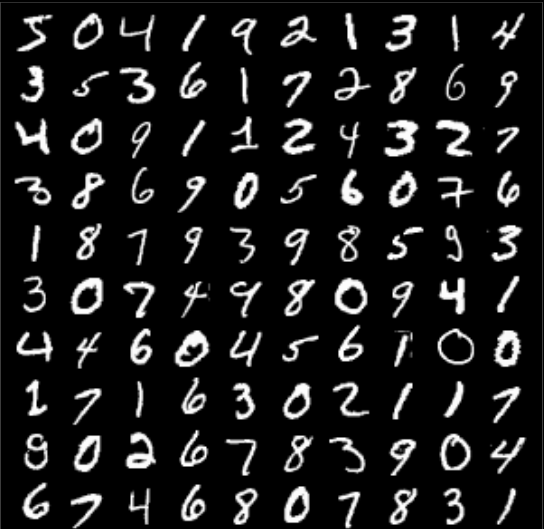
\includegraphics[width=\linewidth]{Figuras/mnist.png}\\[-0.05cm]
\scriptsize Ejemplos de digitos: misma tarea, muchas formas de escribir.
\vspace{0.18cm}
\begin{block}{Pregunta guia}
Si una imagen es una matriz, que perdemos cuando la transformamos en un vector?
\end{block}
\end{columns}
\end{frame}

\begin{frame}[fragile]{Parte 1: cargar y mirar MNIST}
\inputminted[firstline=1,lastline=29]{python}{codes/clase1-p1.py}
\end{frame}

\begin{frame}{De imagen a vector}
\begin{columns}[T,onlytextwidth]
\column{0.38\textwidth}
\begin{itemize}
    \item Una red densa no ve filas, columnas ni vecindad.
    \item \texttt{Flatten} transforma $28\times28$ en $784$ entradas.
    \item La red aun puede aprender patrones, pero debe reconstruir relaciones espaciales desde cero.
\end{itemize}
\column{0.58\textwidth}
\centering
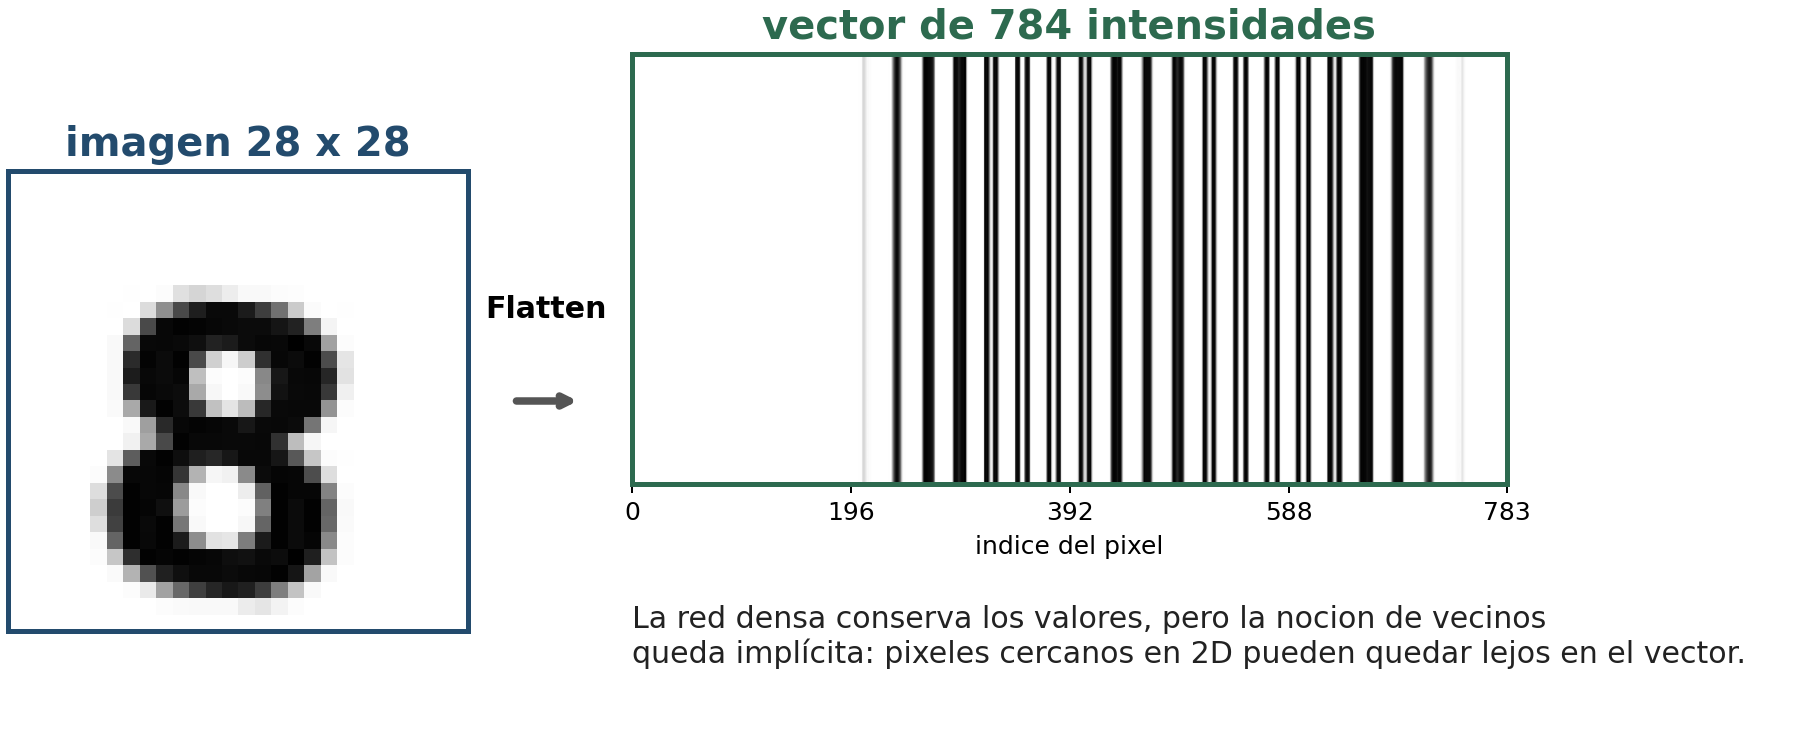
\includegraphics[width=\linewidth]{Figuras/didacticas/mnist_matrix_flatten.png}
\end{columns}
\end{frame}

\begin{frame}{Dos formas de mirar la misma imagen}
\centering
\resizebox{0.96\linewidth}{!}{\begin{tikzpicture}[scale=0.74,transform shape]
\tikzstyle{box}=[draw,rounded corners=3pt,very thick,align=center,font=\small\bfseries]

\node[box,fill=MidnightBlue!10,minimum width=2.1cm,minimum height=2.1cm] (img1) at (0,0) {$28\times28$\\imagen};
\node[box,fill=ForestGreen!10,minimum width=2.4cm,minimum height=1.1cm] (flat) at (3.2,0) {aplanar\\784 numeros};
\node[box,fill=ForestGreen!18,minimum width=2.2cm,minimum height=1.1cm] (dense) at (6.3,0) {Dense\\ReLU};
\node[box,fill=Crimson!12,minimum width=1.8cm,minimum height=1.1cm] (out1) at (9.1,0) {10 clases};
\draw[->,very thick] (img1) -- (flat);
\draw[->,very thick] (flat) -- (dense);
\draw[->,very thick] (dense) -- (out1);
\node[font=\small\bfseries] at (4.7,1.45) {red densa: pierde la vecindad espacial};

\node[box,fill=MidnightBlue!10,minimum width=2.1cm,minimum height=2.1cm] (img2) at (0,-3.2) {$28\times28$\\imagen};
\node[box,fill=Purple!12,minimum width=2.3cm,minimum height=1.1cm] (conv) at (3.2,-3.2) {Conv2D\\filtros};
\node[box,fill=Purple!20,minimum width=2.3cm,minimum height=1.1cm] (pool) at (6.3,-3.2) {MaxPool\\resumen};
\node[box,fill=Crimson!12,minimum width=1.8cm,minimum height=1.1cm] (out2) at (9.1,-3.2) {10 clases};
\draw[->,very thick] (img2) -- (conv);
\draw[->,very thick] (conv) -- (pool);
\draw[->,very thick] (pool) -- (out2);
\node[font=\small\bfseries] at (4.7,-1.75) {CNN: aprende patrones locales reutilizables};
\end{tikzpicture}
}
\vspace{0.2cm}
\begin{block}{Transicion pedagogica}
La red densa sera nuestra linea base. La CNN aparece como respuesta a una pregunta concreta: como conservar y reutilizar relaciones locales entre pixeles?
\end{block}
\end{frame}

\begin{frame}{Clasificacion multiclase}
\begin{itemize}
    \item La salida tiene 10 neuronas, una por digito.
    \item \texttt{softmax} convierte puntajes en probabilidades aproximadas.
    \item La perdida \texttt{sparse\_categorical\_crossentropy} compara la clase real con la distribucion predicha.
    \item \texttt{accuracy} mide fraccion de aciertos, pero no dice que digitos se confunden.
\end{itemize}
\begin{alertblock}{Lectura responsable}
Una probabilidad alta significa que el modelo es confiado, no necesariamente que tenga razon.
\end{alertblock}
\end{frame}

\begin{frame}[fragile]{Parte 2: red densa simple}
\inputminted{python}{codes/clase1-p2.py}
\end{frame}

\begin{frame}{Actividad de interpretacion}
\begin{block}{Trabajo en parejas}
Antes de pasar a la CNN, observar ejemplos mal clasificados y responder:
\end{block}
\begin{itemize}
    \item Que digitos se confunden con mayor frecuencia?
    \item El error parece venir de escritura ambigua o del modelo?
    \item Que informacion local de la imagen seria util conservar?
    \item Que esperarian que mejore una CNN?
\end{itemize}
\end{frame}

\begin{frame}[fragile]{Parte 3: mirar errores de la red densa}
\inputminted{python}{codes/clase1-p3.py}
\end{frame}

\begin{frame}{Leer errores, no solo accuracy}
\begin{columns}[T,onlytextwidth]
\column{0.50\textwidth}
\begin{itemize}
    \item La matriz de confusion muestra que clases se confunden.
    \item La diagonal resume aciertos; los valores fuera de la diagonal son errores especificos.
    \item Para discutir modelos de imagenes conviene mirar ejemplos, no solo promedios.
\end{itemize}
\begin{alertblock}{Pregunta para la sala}
Si el modelo confunde 4 con 9, que parte visual del digito deberiamos inspeccionar?
\end{alertblock}
\column{0.46\textwidth}
\centering
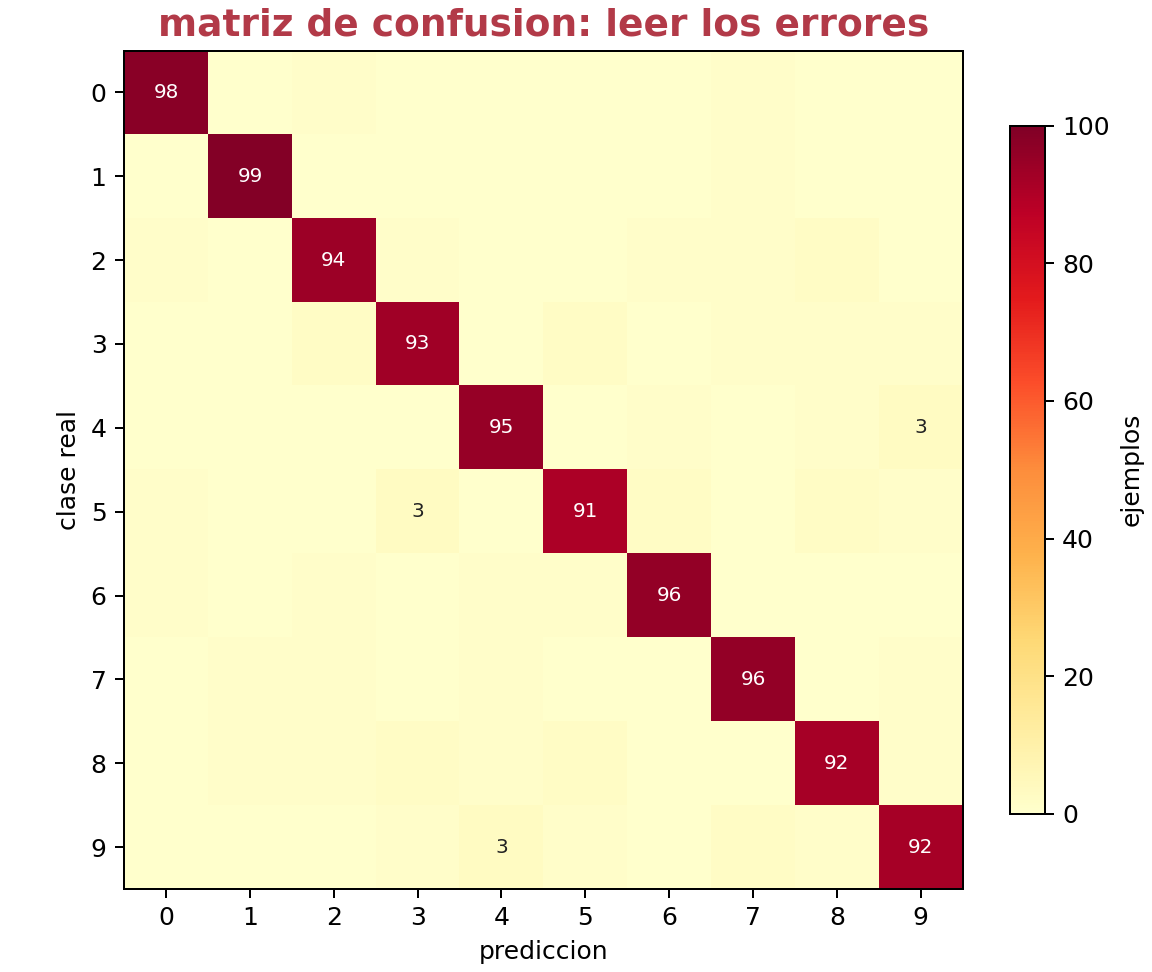
\includegraphics[width=\linewidth,height=0.70\textheight,keepaspectratio]{Figuras/didacticas/confusion_matrix_example.png}
\end{columns}
\end{frame}

\begin{frame}{Cierre Clase 1}
\begin{itemize}
    \item Una red densa es una linea base razonable para MNIST.
    \item Aplanar una imagen simplifica el problema, pero elimina la estructura espacial explicita.
    \item Los errores concretos preparan la pregunta de la Clase 2: como usar la geometria local de los pixeles?
\end{itemize}
\end{frame}

\section{Clase 2}

\begin{frame}[plain]
\centering
\vfill
{\Huge \bfseries Clase 2}\\[0.4cm]
{\Large Redes convolucionales y fotografias propias}
\vfill
\end{frame}

\begin{frame}{Objetivos de la Clase 2}
\begin{itemize}
    \item Construir una CNN pequena con \texttt{Conv2D} y \texttt{MaxPooling2D}.
    \item Comparar validacion y test contra la red densa de la Clase 1.
    \item Interpretar convoluciones como detectores de patrones locales.
    \item Probar el modelo con una fotografia tomada por estudiantes.
    \item Discutir por que el rendimiento baja al salir del dataset limpio.
\end{itemize}
\end{frame}

\begin{frame}{Que hace una convolucion}
\begin{columns}[T,onlytextwidth]
\column{0.42\textwidth}
\small
\begin{itemize}
    \item Un filtro pequeno recorre la imagen.
    \item El mismo filtro se reutiliza en distintas posiciones.
    \item Las primeras capas pueden detectar bordes, trazos o esquinas.
    \item El pooling resume regiones y reduce sensibilidad a desplazamientos pequenos.
\end{itemize}
\textbf{Idea computacional:} la CNN aprende patrones locales que pueden aparecer en muchas zonas.
\column{0.54\textwidth}
\centering
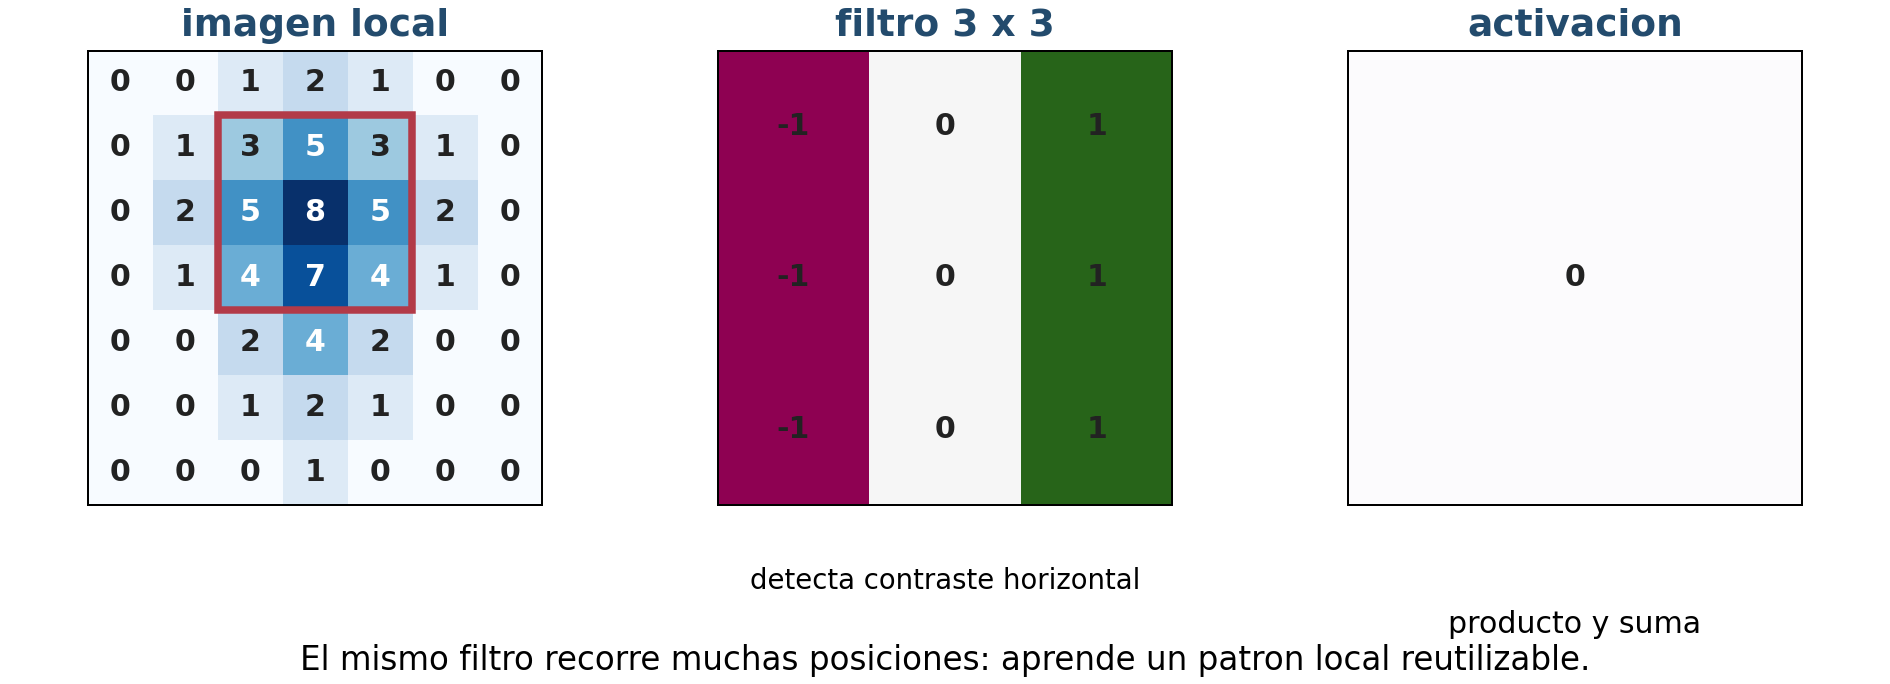
\includegraphics[width=0.94\linewidth]{Figuras/didacticas/convolution_window.png}
\end{columns}
\end{frame}

\begin{frame}{Del filtro al clasificador}
\centering
\resizebox{0.96\linewidth}{!}{\begin{tikzpicture}[scale=0.76,transform shape]
\tikzstyle{box}=[draw,rounded corners=3pt,very thick,minimum width=2.05cm,minimum height=1.0cm,align=center,font=\small\bfseries]
\node[box,fill=MidnightBlue!12] (input) at (0,0) {entrada\\$28\times28\times1$};
\node[box,fill=Purple!12] (conv1) at (2.8,0) {Conv2D\\8 filtros};
\node[box,fill=Purple!18] (pool1) at (5.6,0) {MaxPool\\$2\times2$};
\node[box,fill=Purple!12] (conv2) at (8.4,0) {Conv2D\\16 filtros};
\node[box,fill=ForestGreen!14] (dense) at (11.2,0) {Dense\\64};
\node[box,fill=Crimson!12,minimum width=1.8cm] (out) at (13.8,0) {softmax\\10};
\foreach \a/\b in {input/conv1,conv1/pool1,pool1/conv2,conv2/dense,dense/out} {
  \draw[->,very thick,gray!75] (\a) -- (\b);
}
\node[font=\scriptsize,align=center,text width=12.0cm] at (6.9,-1.35) {Las primeras capas no deciden el digito completo: detectan trazos simples. Las capas finales combinan esos trazos para clasificar.};
\end{tikzpicture}
}
\vspace{0.25cm}
\begin{block}{Lectura por capas}
Las primeras capas responden a trazos simples. Las capas finales combinan esos trazos para decidir entre las 10 clases.
\end{block}
\end{frame}

\begin{frame}{Arquitectura propuesta}
\begin{columns}[T,onlytextwidth]
\column{0.45\textwidth}
\begin{itemize}
    \item Entrada: imagen $28\times28\times1$.
    \item Bloque 1: convolucion con pocos filtros y pooling.
    \item Bloque 2: otra convolucion y pooling.
    \item Clasificador final: \texttt{Flatten}, \texttt{Dense}, \texttt{softmax}.
\end{itemize}
\begin{alertblock}{Escala docente}
La red es intencionalmente pequena. Queremos que entrene rapido durante la clase y que la mejora conceptual sea visible.
\end{alertblock}
\column{0.51\textwidth}
\centering
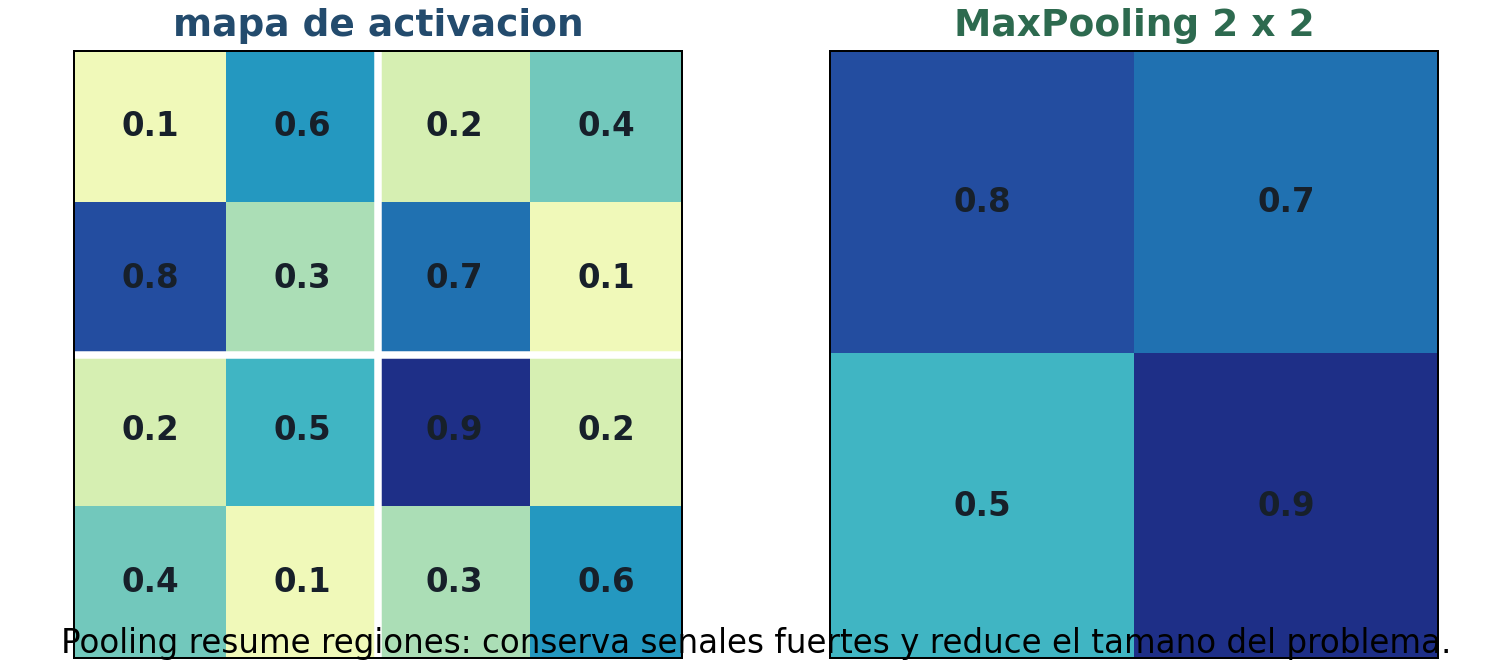
\includegraphics[width=\linewidth]{Figuras/didacticas/pooling_demo.png}
\end{columns}
\end{frame}

\begin{frame}[fragile]{Parte 1: entrenar una CNN}
\inputminted{python}{codes/clase2-p1.py}
\end{frame}

\begin{frame}{Comparacion justa}
\begin{itemize}
    \item Usamos el mismo train, validation y test.
    \item No cambiamos la pregunta: seguimos clasificando digitos.
    \item Cambiamos la arquitectura para aprovechar estructura espacial.
    \item La comparacion debe hacerse con metricas y ejemplos, no solo con una sensacion visual.
\end{itemize}
\end{frame}

\begin{frame}[fragile]{Parte 2: red densa versus CNN}
\inputminted{python}{codes/clase2-p2.py}
\end{frame}

\begin{frame}{De MNIST a una foto real}
\begin{columns}[T,onlytextwidth]
\column{0.43\textwidth}
\begin{itemize}
    \item La foto puede tener sombras, fondo irregular, rotacion y grosor distinto.
    \item Hay que convertirla a escala de grises, invertir si hace falta y llevarla a $28\times28$.
    \item El modelo no ``ve'' una foto: ve un arreglo numerico parecido al formato de entrenamiento.
\end{itemize}
\column{0.53\textwidth}
\centering
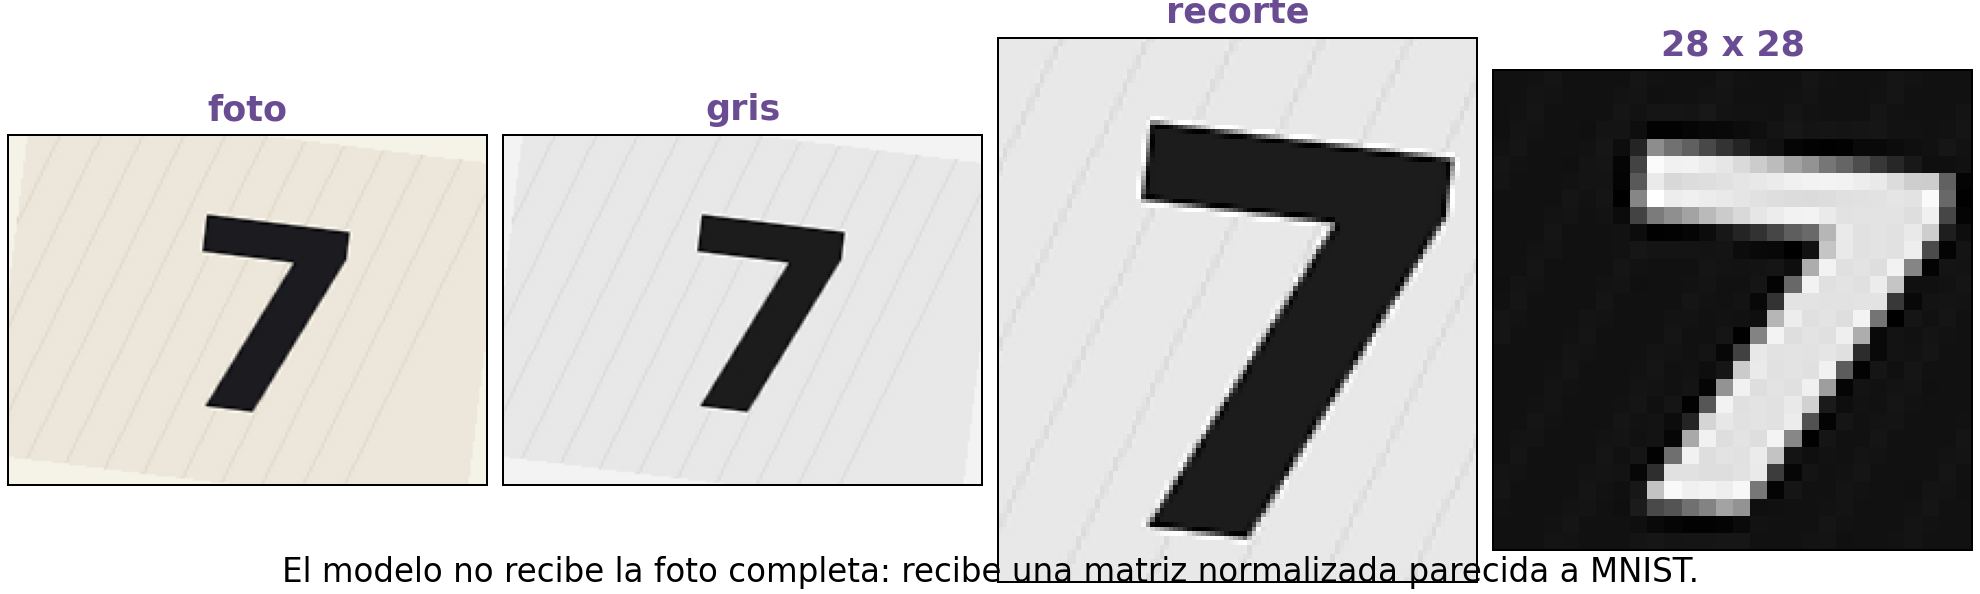
\includegraphics[width=\linewidth]{Figuras/didacticas/photo_preprocess_pipeline.png}
\vspace{0.12cm}
\begin{block}{Actividad}
Cada grupo fotografia un numero escrito en papel, lo procesa con el codigo y observa la prediccion de la red que entreno.
\end{block}
\end{columns}
\end{frame}

\begin{frame}{Cuando una prediccion falla}
\begin{columns}[T,onlytextwidth]
\column{0.48\textwidth}
\begin{block}{Revisar el dato}
Antes de culpar a la arquitectura, mirar contraste, centrado, tamano del digito, sombras y orientacion.
\end{block}
\column{0.48\textwidth}
\begin{alertblock}{Revisar el modelo}
Despues comparar confianza, matriz de confusion y ejemplos parecidos del set de entrenamiento.
\end{alertblock}
\end{columns}
\vspace{0.25cm}
\begin{itemize}
    \item El error puede venir del preprocesamiento, de la escritura o de una limitacion real del modelo.
    \item Esta separacion ayuda a pensar como cientificos computacionales: dato, modelo y validacion se revisan juntos.
\end{itemize}
\end{frame}

\begin{frame}[fragile]{Parte 3: fotografiar un numero}
\inputminted{python}{codes/clase2-p3.py}
\end{frame}

\begin{frame}{Actividad breve: hacer el problema mas realista}
\begin{block}{Experimentos sugeridos}
Cambiar un aspecto a la vez y observar la prediccion:
\end{block}
\begin{itemize}
    \item escribir el numero mas delgado o mas grueso;
    \item tomar la foto con fondo claro y luego con sombras;
    \item rotar levemente el papel;
    \item probar numeros ambiguos, por ejemplo 1/7 o 4/9;
    \item comparar red densa y CNN sobre la misma foto procesada.
\end{itemize}
\end{frame}

\begin{frame}[fragile]{Parte 4 opcional: aumento de datos}
\inputminted{python}{codes/clase2-p4.py}
\end{frame}

\begin{frame}{Preguntas para guiar la discusion}
\begin{itemize}
    \item Por que una CNN suele generalizar mejor que una red densa en imagenes?
    \item Que transformaciones de la foto destruyen informacion importante?
    \item Que significa que el modelo entregue una confianza alta en una foto mal procesada?
    \item Como cambiaria el problema si las imagenes fueran galaxias, crateres o microestructuras?
    \item Que pasos agregariamos antes de usar esto en una aplicacion cientifica real?
\end{itemize}
\end{frame}

\begin{frame}{Cierre de la semana}
\begin{itemize}
    \item La red densa entrega una base clara: la imagen puede tratarse como vector, pero se pierde vecindad espacial.
    \item La CNN introduce filtros locales reutilizables, una idea especialmente natural para imagenes cientificas.
    \item Probar con una foto propia revela la diferencia entre datos de laboratorio docente y datos reales.
    \item La arquitectura mejora el modelo, pero el preprocesamiento y la validacion siguen siendo parte central del trabajo computacional.
\end{itemize}
\end{frame}

\end{document}
